%%quellen
%% http://www.raspbian.org/RaspbianDocumentation
%% http://www.raspberrypiguide.de
%% http://www.raspberrypi.org
%%
%% Beuth Hochschule für Technik --  
%%
%% Kapitel 2 - Raspberry Pi
%%
%%	
\chapter{Raspberry Pi}

\lstset{language=C,
				backgroundcolor=\color{light-gray},
				%frame=single,
				tabsize=2,
				%numbers=left,
				numbersep=5pt,
				%numberstyle=\color{light-gray},
				basicstyle=\ttfamily\color{black}\small,
				keywordstyle=\color{HKS51}\bfseries,
				commentstyle=\color{HKS13}\slshape,,
				identifierstyle=\color{blue},
				stringstyle =\color{orange}}

\begin{figure}[h]
  \begin{center}		%width=\linewidth
    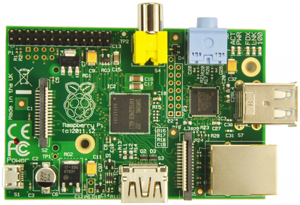
\includegraphics[scale=0.6]{raspberrypi-model-b.png}
  		  \caption{Raspberry Pi Model B}
     \label{raspPic}
  \end{center}
\end{figure}			
				
Das Raspberry Pi ist ein kreditkartengroßer Einplatinencomputer von der \textit{Raspberry Pi Foundation}\footnote{Stiftung und Wohltätigkeitsorganisation in Großbritannien} entwickelt wurde. Mithilfe seiner 700 MHz starken ARM-CPU kann er nahezu alles was auch normale Desktoprechner können.\\

Ziel der Entwicklung des Raspberry Pi ist das Interesse an dem Studium der Informatik und ähnliche Fachgebiete zu fördern, bzw. einen günstigen Computer zum Programmieren und Experimentieren anbieten zu können.\\

Durch die geringe Leistungsaufnahme, günstigen Preis und viele verschiedene Ausbau- und Personalisierungsmöglichkeiten können Raspberry Pi’s für verschiedene Zwecke eingesetzt werden. Unter anderem sind beliebte Projekte für den Haushalt Wetterstationen, Radiosender, Media Center, NAS, etc.

\newpage

%%%%%%%%%%%%%%%%%%%%%%%%%%%%%%%%%%%%%%%%%%%%%%%%%%%%%%%%%%%%%%%%%%%%%%
\section{Hardware}
%%-------------------------------------------------------------------
\subsection{Technische Spezifikationen}

\begin{figure}[h]
  \begin{center}		%width=\linewidth
    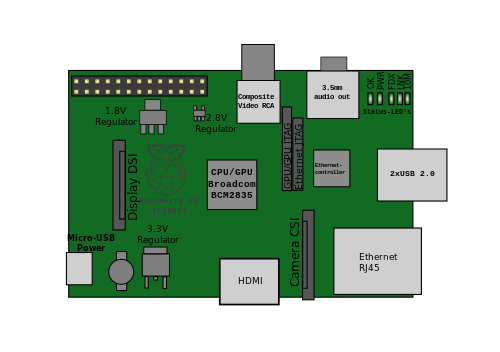
\includegraphics[scale=0.6]{overview.png}
  		  \caption{Raspberry Pi Model B Komponenten}
     \label{raspPic_Komp}
  \end{center}
\end{figure}

\begin{longtable}{||l|l||}

\hline
Komponente & Kenndaten\\ \hline\hline
\endfirsthead
\hline
Komponente & Kenndaten \\ \hline\hline
\endhead

Größe & 85,60 x 53,98 x 17 mm\\ \hline
Soc & Broadcom BCM2835\\ \hline
CPU & ARM1176JZF-S(700MHz)\\ \hline
GPU & Broadcom VideoCore IV \\ \hline
SDRAM & 512MB\\ \hline
USB 2.0 & 2\\ \hline
Videoausgabe & HDMI \& S-Video\\ \hline
Tonausgabe & 3,5mm Klinkenstecker \& HDMI\\ \hline
Speicher & SD(SDHC/SDXC)/MMC/SDIO Kartenleser bis 128GB\\ \hline
Netzwerk & 10/100 MBit Ethernet\\ \hline
Schnittstellen & 17 GPIO-Pins, SPI, 21C, UART\\ \hline
Stromversorgung & 5V Micro-USB Anschluss\\ \hline

\end{longtable}
\footnote{http://www.raspberrypiguide.de; http://www.raspberrypi.org; 15.01.2014}


\newpage

%%-------------------------------------------------------------------
\subsection{Kamera}

\begin{figure}[h]
  \begin{center}		%width=\linewidth
    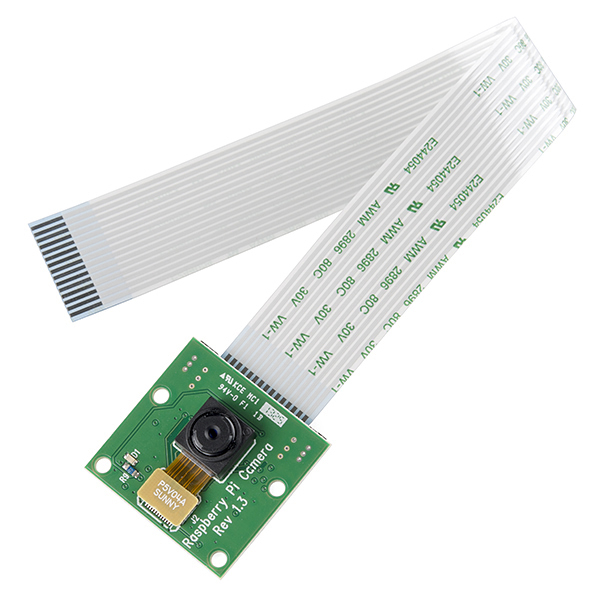
\includegraphics[scale=0.3]{camera.jpg}
  		  \caption{Raspberry Kamera}
     \label{raspCam}
  \end{center}
\end{figure}


\begin{longtable}{||l|l||}

\hline
Komponente & Kenndaten\\ \hline\hline
\endfirsthead
\hline
Komponente & Kenndaten \\ \hline\hline
\endhead

Größe & 20 x 24 mm\\ \hline
Sensor & OmniVision OV5647 (5MP)\\ \hline
Auflösung & 2592 x 1944\\ \hline
Video & 1080p \@ 30fps \\ \hline
Anschluss & 15-Pin Flachbandkabel\\ \hline

\end{longtable}

Die Kamera wurde speziell für den Raspberry Pi entwickelt, diese wird an die CSI-Schnittstelle (Camera Serial Interface) des Pi angeschlossen. Anschließend muss die Kamera-Unterstützung mittels des Konfigurationsprogramms \texttt{raspi-config} noch aktiviert werden.

\newpage

%%%%%%%%%%%%%%%%%%%%%%%%%%%%%%%%%%%%%%%%%%%%%%%%%%%%%%%%%%%%%%%%%%%%%%
\section{Software und Einstellungen}

%%-------------------------------------------------------------------
\subsection{Betriebssystem}
Für das Raspberry Pi worden mehrere Open Source Betriebssysteme programmiert. Alle basieren auf verschiedene Linux Distributionen(u.a. OpenSUSE, Fedora, FreeBSD, Debian). Je nach Bedarf kann sich jeder Nutzer für eine Distribution entscheidend. Eins der beliebtestens Distrubutionen ist Raspbian, basierend auf Debian, was auch in diesem Projekt benutzt wird. Raspbian inkludiert alle Grundprogramme und -Utilities, dass mit vielen verschiedenen Packages kompatibel sind. Dieser Betriebssystem hat sich im laufe der Zeit als sehr stabil bewiesen.\\

Es gibt auch die Möglichkeit Windows auf das Raspberry Pi zu installieren, obwohl Nutzer davon abgeraten werden. Das Windows Betriebssystem benötigt zu viele Ressourcen und läuft sehr langsam und instabil auf das Raspberry Pi.\\

Andere Distributionen sind Gebrauchorientiert aufgestellt, wie zum Beispiel für Media Center das beliebte XBMC (OpenELEC, Raspbmc, XBian). Weiterhin gibt es auch Androidsysteme, die auf das Raspberry Pi portiert worden sind.
\footnote{http://www.raspbian.org; 15.01.2014}


%%-------------------------------------------------------------------
\subsection{LAMP Webserver}
LAMP steht für Linux Apache MySQL PHP Webserver. Auf das Raspberry Pi wurde ein LAMP Server installiert, um die Desktop/Mobil Applikation mit dem Pi zu verbinden und Informationen auszutauschen. Durch die Einstellung eines DNS kann auf das Videostreams sowie auf die MySQL Datenbank zugegriffen werden. Damit \textit{http} oder \textit{ssh} Anfragen  an das Server im Raspberry Pi ankommen, müssen Ports für die Verbindung zur Verfügung gestellt werden. Im diesen Fall muss jeweils ein Port für die SSH-Verbindung, den Videostream und die Datenbankzugriffe freigegeben werden.\\

Um das LAMP Webserver zu installieren werden folgende Kommandos mit Administratorrechte ausgeführt:\\
\begin{lstlisting}
apt-get install apache2
apt-get install mysql-server
sudo apt-get install php5
sudo apt-get install php5-mysql
\end{lstlisting}

%%-------------------------------------------------------------------
\subsection{SSH Zugriff}
Damit das Team gleichzeitig auf das Raspberry Pi arbeiten konnte wurde auf das System eine SSH-Verbindung eingestellt. So wurden auch Entwicklungskosten gespart, weil nicht jeder Teammitglied ein System benötigte.\\

Um das Raspberry Pi per Fernzugriff zu betreiben ist es nötig eine \textit{Secure Shell} Verbindung aufzubauen. Durch die Verfügung einer SSH-Verbindung können Updates, Support und Wartungsarbeiten per Fernzugriff auf das System ausgeübt werden, dieses spart kosten für den Kunden sowie für den Support.

Als Sicherheitsmaßnahmen wurde der Standardport für SSH-Verbindungen (Port 22) auf ein anderen Port geändert und eine Public Key Authentifizierung implementiert. Um den Port für die SSH-Verbindung zu ändern, muss in der Datei \textit{/etc/ssh/sshd\_config} der Wert \textit{\#Port} auf den gewünschten Wert gesetzt werden. Danach muss das Dienst neu gestartet werden und somit ist der neue Port eingestellt.\\

Die Public Key Authentifizierung erfolgt indem der Benutzer ein privaten und einen öffentlichen Schlüssel erstellt. Der private Schlüssel wird am Client gespeichert und der öffentlicher Schlüssel am Server. Mit dem Befehl

\begin{lstlisting}
ssh-keygen -t dsa
\end{lstlisting}

werden die Schlüsseln generiert. Hier muss der Benutzer ein Passwort eingeben, mit dem sich er am Server anmelden wird. In der Regel heißen beider Schlüssel \textit{id\_das} und \textit{id\_das.pub}. Der private Schlüssel muss an das Client bekannt gemacht werden, indem man in der \textit{/ssh2/identification} Datei die Zeile 

\begin{lstlisting}
idkey id_dsa
\end{lstlisting}

bearbeitet oder einbaut. Der Inhalt des öffentlichen Schlüssels muss in der Datei \textit{/ssh/authorized\_keys} hinzugefügt werden.

\begin{lstlisting}
cat new_key.pub >> .ssh/authorized_keys
\end{lstlisting}

Jetzt ist der Client und der Server so konfiguriert, dass nur Rechner mit dem privaten Schlüssel Zugriff auf den Server haben über den konfigurierten Port.
Eine SSH-Verbindung wird mit folgendermaßen aufgebaut:
\begin{lstlisting}
ssh -p XXXX benutzer@serverAdresse
\end{lstlisting}

%%-------------------------------------------------------------------
\subsection{DNS}
Um das Raspberry Pi über das lokale Netz erreichbar zu machen, wurde erstmal ein Webserver aufgebaut. Um jetzt das System überall über das Internet erreichbar ist, muss eine Domain reserviert werden. Somit kann ein Benutzer Zugriffe auf die Datenbank, sowie auf das Videostream aus jedem Rechner oder Android Mobilgerät weltweit ausüben. Der Dienst ``no ip'' bietet solche Dienstleistung kostenlos an. Für dieses Projekt wurde die Adresse \textit{spyhole.no-ip.biz} eingestellt und durch die Freigabe und Weiterleitung von Ports können die programmierten Applikationen auf das Raspberry Pi zugreifen.\\

Da dieses Projekt im eine privaten Haushalt verwendet wird, besitzt in der Regel der Benutzer keine feste IP Adresse. Deswegen muss die IP Adresse hinter des DNS zyklisch geprüft werden. Der Dienst ``no ip'' stellt ein Programm zur Verfügung, das sich um die Überprüfung der Gültigkeit der IP Adresse kümmert. Das Programm muss dann mit den Kommandos

\begin{lstlisting}
make
make install
\end{lstlisting}

installiert werden. Während der Installation wird von den Benutzer das Login, Passwort und die Aktualisierungszeit verlangt. Danach wird der Dienst mit

\begin{lstlisting}
/usr/local/bin/noip2
\end{lstlisting}

gestartet. Der Dienst läuft bis das System runter gefahren wird. Daher ist es ratsam der Dienst im \textit{/etc/init.d} einzutragen.

%%%%%%%%%%%%%%%%%%%%%%%%%%%%%%%%%%%%%%%%%%%%%%%%%%%%%%%%%%%%%%%%%%%%%%
\subsection{Datenbanken}
Hier wird über die Datenbank und der Aufbau der Tabellen beschrieben. Als Datenbank benutzen wir MySQL-Server zur Speicherung der Daten. Zur Verwaltung der Daten in der Datenbank verwenden wir das Tool \texttt{phpMyAdmin}.

\subsubsection{Was ist SQL ?}
SQL ist einer der verbreitetsten Standards, um eine Kommunikation zwischen Server und Client mit Datenbanken zu ermöglichen. Mit SQL ist es möglich, Daten aus einer Datenbank zu selektieren, einzutragen, zu aktualisieren und zu löschen. Auch besteht die Möglichkeit mit Hilfe der SQL Tabellen in einer Datenbank zu erstellen, zu modifizieren oder zu löschen. Integriert ist ebenfalls eine Zugriffsverwaltung auf die Tabellen. 

Das Schema der Datenbank legt fest, welche Daten in einer Datenbank in welcher Form gespeichert werden können und welche Beziehungen zwischen den Daten bestehen. Insbesondere bei relationalen Datenbanken legt das Schema die Tabellen und deren Attribute sowie zur Sicherstellung der Konsistenz die Integritätsbedingungen fest. Dabei wird auch speziell der Primärschlüssel bzw. die Eindeutigkeitsbedingungen festgelegt.

\subsubsection{Was ist phpMyAdmin ?}
\texttt{phpMyAdmin} ist ein freies praktisches PHP-Tool zur Verwaltung von MySQL-Datenbanken. Das Tool bietet die Möglichkeit über HTTP mit einem Browser in MySQL neue Datenbanken zu erstellen bzw. zu löschen. Des Weiteren erlaubt das Tool die Erstellung, Löschung und Veränderung von Tabellen und Datensätzen. Auch die Verwaltung von Schlüssel-Attributen ist implementiert. Eine Anwendungsmöglichkeit des Tools \texttt{phpMyAdmin} ist die SQL-Statements direkt auszuführen und somit eine ausführliche grafische Abfrage der vorhandenen Daten in Form von Tabellen darzustellen. Für die Bedienung des Tools sind kaum Kenntnisse in SQL erforderlich, da das Tool nach dem WYSIWYG\footnote{ist das Akronym für das Prinzip „\textbf{W}hat \textbf{Y}ou \textbf{S}ee \textbf{I}s \textbf{W}hat \textbf{Y}ou \textbf{G}et“ (deutsch „Was du siehst, ist was du bekommst.“).} - Prinzip arbeitet.

\subsubsection{Aufbau}
\lstset{language=SQL,
				backgroundcolor=\color{light-gray},
				%frame=single,
				tabsize=2,
				%numbers=left,
				numbersep=5pt,
				%numberstyle=\color{light-gray},
				basicstyle=\ttfamily\color{black}\small,
				keywordstyle=\color{HKS51}\bfseries,
				commentstyle=\color{HKS13}\slshape,,
				identifierstyle=\color{blue},
				stringstyle =\color{orange}}
				
Die Datenbank \texttt{db\_spyhole} besteht aus drei Tabellen (tb\_doorloggers, tb\_users und tb\_images). In der  Tabelle \texttt{tb\_doorloggers} werden die Aktivitäten an der Tür gespeichert \textbf{(?)}, in der Tabelle \texttt{tb\_users} sind die registierte Users gespeichert, und die Tabelle \texttt{tb\_images} dient zur Speicherung der Bilder \textbf{(welche Bilder? Kommt noch dazu}).  

Ich werde den Aufbau der drei Tabellen genauer beschreiben:
\lstset{language=SQL,
				backgroundcolor=\color{light-gray},
				%frame=single,
				tabsize=2,
				breaklines=true,
				%numbers=left,
				numbersep=5pt,
				%numberstyle=\color{light-gray},
				basicstyle=\ttfamily\color{black}\small,
				keywordstyle=\color{HKS51}\bfseries,
				commentstyle=\color{HKS13}\slshape,,
				identifierstyle=\color{blue},
				stringstyle =\color{orange}}
\begin{lstlisting}[caption={Aufbau der Datenbanktabellen},captionpos=b]
--
-- Tabellenstruktur für Tabelle `tb_doorlogger`
--

CREATE TABLE IF NOT EXISTS `tb_doorlogger` (
  `ID` int(8) NOT NULL AUTO_INCREMENT,
  `U_ID` int(8) NOT NULL,
  `date` datetime NOT NULL,
  PRIMARY KEY (`ID`)
) ENGINE=InnoDB DEFAULT CHARSET=utf8 COLLATE=utf8_unicode_ci AUTO_INCREMENT=1 ;
-- --------------------------------------------------------

--
-- Tabellenstruktur für Tabelle `tb_images`
--

CREATE TABLE IF NOT EXISTS `tb_images` (
  `ID` int(8) NOT NULL AUTO_INCREMENT,
  `dl_ID` int(8) NOT NULL,
  `U_ID` int(8) NOT NULL,
  `imgdata` longblob,
  `imgtype` varchar(32) COLLATE utf8_unicode_ci DEFAULT NULL,
  PRIMARY KEY (`ID`)
) ENGINE=InnoDB DEFAULT CHARSET=utf8 COLLATE=utf8_unicode_ci AUTO_INCREMENT=1 ;

-- --------------------------------------------------------

--
-- Tabellenstruktur für Tabelle `tb_user`
--

CREATE TABLE IF NOT EXISTS `tb_user` (
  `ID` int(8) NOT NULL AUTO_INCREMENT,
  `name` varchar(64) COLLATE utf8_unicode_ci NOT NULL,
  `firstname` varchar(64) COLLATE utf8_unicode_ci NOT NULL,
  `email` varchar(128) COLLATE utf8_unicode_ci NOT NULL,
  `user` varchar(16) COLLATE utf8_unicode_ci NOT NULL,
  `password` varchar(255) CHARACTER SET utf8 COLLATE utf8_bin NOT NULL,
  `u_timestamp` timestamp NOT NULL DEFAULT '0000-00-00 00:00:00' ON UPDATE CURRENT_TIMESTAMP,
  PRIMARY KEY (`ID`)
) ENGINE=InnoDB DEFAULT CHARSET=utf8 COLLATE=utf8_unicode_ci AUTO_INCREMENT=1 ;

\end{lstlisting}
Das Attribut „ID“ vom Typ „INT“ kann Werte von  -2147483648 bis 2147483647 erfassen. Die Attribute vom Typ „VARCHAR()“ können beliebige Zeichenkombinationen speichern. Die maximale Zeichenlänge ist dabei von der in der Klammer befindlichen Zahl abhängig. Der Befehl „NOT NULL“ in der Definition der Attribute bewirkt, dass die entsprechende Spalte mit Daten vorhanden sein muss, sobald ein neuer Datensatz angelegt wird. Anders sieht es aber beim Befehl „DEFAULT NULL“ aus, dass die entsprechende Spalte nicht zwingend mit Daten gefüllt werden muss und standardmäßig auf NULL gesetzt wird, wenn ein neuer Datensatz keine Daten enthält. Das Attribut „ID“ wird als Primärschlüssel (Befehl „PRIMARY KEY (`ID`)“ definiert und mit AUTO\_INCREMENT zusätzlich ausgestattet. Das hat die folgende Bedeutung, dass das Attribut „ID“ fortlaufend um eins erhöht wird, wenn ein neuer Datensatz hinzufügt wird. Ein Primärschlüssel dient der eindeutigen Identifizierung der einzelnen Zeilen in einer Tabelle. 

%%%%%%%%%%%%%%%%%%%%%%%%%%%%%%%%%%%%%%%%%%%%%%%%%%%%%%%%%%%%%%%%%%%%%%
\section{OpenCV und Gesichtserkennung}

Ist eine freie Programmbibliothek(unter BSD-Lizens) mit Algorithmen für Bildverarbeitung und maschinelles sehen. Es beinhaltet C/C++, Python und Java Interfaces und unterstützt Windows, Linux, Mac OS, iOS and Android. OpenCV wird sowohl im kommerziellen wie im privaten Bereich stark benutzt.\footnote{http://opencv.org; 02.02.2014}\\

Unter die vielen Möglichkeiten das OpenCV anbietet, ist für dieses Projekt die Funktionen der Gesichtserkennung relevant. Um Bewegungen und Gesichter zu erkennen, muss die Aufnahme der Kamera in drei Schritte auswertet werden. 


\subsection{Logarithmus traineren}
Unter Logarithmus trainieren wird gemeint, den Gesichtserkennungsalgorithmus wird bekannt gemacht anhand vorhandenen Bilder, welche Personen identifiziert werden. Dafür müssen Bilder von den jeweiligen Personen im System gespeichert sein. Um eine höhere Übertragungsrate zu erreichen werden die Bilder der Kamera nur in Schwarz-Weiß aufgenommen. Deswegen müssen die Trainingsbilder im gleichen Format vorliegen. Mittels eines C-Programmes werden die Gesichter geschnitten und in einen neuen Schwarz-Weiß Bild gespeichert.\\

\begin{figure}[h]
  \begin{center}		%width=\linewidth
    
\includegraphics{matthias4.jpg}
  		  \caption{Trainingsbild}
     \label{Trainingsbild}
  \end{center}
\end{figure}

\newpage
Mittels einer csv-Datei wird zu jeder Person eine Identifikationsnummer zugewiesen und dem Hauptprogramm bekannt gegeben, wo diese Bilder gespeichert sind. Zum Beispiel:\\

\begin{lstlisting}
/home/pi/pictures/Person1.jpg;1
/home/pi/pictures/Person2.jpg;2
/home/pi/pictures/Person3.jpg;3
\end{lstlisting}


%%-------------------------------------------------------------------
\subsection{Kamera Initializieren}
Videos sind die Wiedergabe von einer Bildersequenz, also werden einzelne Bilder bearbeitet und ausgewertet.  Zuerst wird die angeschlossene Webcam angesprochen und die Videoaufnahme gestartet. Dies folgt dem gleichen Prinzip wie eine Datei öffnen und aus dieser Datei Zeilenweise lesen. Jede gelesene Zeile wird gespeichert und von einem andere Algorithmus bearbeitet. Bei der Webcam werden einzelne Bilder gespeichert und danach bearbeitet.\\
 
\subsection{Bild auswerten}
 Wenn ein Bild gespeichert worden ist, kann dieser ausgewertet werden. Als erstes wird versucht, mittels OpenCV, ein Gesicht im das jeweilige Bild zu erkennen. Ist dieser Schritt erfolgreich, wird um das erkannte Gesicht ein Viereck gezeichnet. Danach versucht das Algorithmus anhand der mit der csv-Datei ausgewertete Bilder, festzustellen ob diese Person bekannt ist. Falls ja, wird anhand der Identifikationsnummer ein Name (im Programmcode fest kodiert) hinzugefügt. \\


\begin{figure}[h]
  \begin{center}		%width=\linewidth
    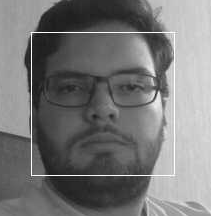
\includegraphics[scale=0.5]{unknown.png}
  		  \caption{Nicht erkannte Person}
     \label{unknown}
  \end{center}
\end{figure}

Dieses bearbeitetes Bild wird für die Ausgabe über den Streamer gespeichert. Der Streamer liest das bereits ausgewertete Bild nach der Gesichtserkennung und stellt es als Stream zur Verfügung.
 
 
%%%%%%%%%%%%%%%%%%%%%%%%%%%%%%%%%%%%%%%%%%%%%%%%%%%%%%%%%%%%%%%%%%%%%%
\section{MJPG Streamer}
MJPG-Streamer bittet die Möglichkeit Videodaten von einer Videoquelle als Motion-JPEG streamen zu lassen. Modernere Netzwerkkameras erzeugen Videostreams automatisch, während mit Hilfe von diesem Programm, auch einfache Webcams an einem Rechner mit Internet-Zugang Streams erzeugen können. MJPG Streamer gehört nicht zu den offiziellen Paketen von Linux und muss manuell kompiliert werden. Dafür sind folgende Pakete nötig:

\begin{itemize}
  \item build-essential
  \item libjpeg-dev
  \item imagemagick
  \item subversion
\end{itemize}

Das aktuelle Quellcode muss von der Webseite \textit{http://sourceforge.net/projects/mjpg-streamer/} heruntergeladen werden und dementsprechend kompiliert werden.\footnote{http://sourceforge.net/apps/mediawiki/mjpg-streamer/index.php?title=Main\_Page; 02.02.2014} Über einem Webbrowser hat man Zugriff auf das Stream. Im diesem Projekt lautet die Adresse für das Stream \textit{spyhole.no-ip:1900}(der Default Port 8080 wurde auf 1900 geändert). Hier wird eine Oberfläche mit verschiedenen Streamoptionen dargestellt. Unter anderem Java und Javascript, sowie die Möglichkeit das Stream mittels das Programm VLC zu sehen. Durch Personalisieren dieser Webseite haben unsere Desktop und Mobile App zugriff auf das Stream.
